% Options for packages loaded elsewhere
\PassOptionsToPackage{unicode}{hyperref}
\PassOptionsToPackage{hyphens}{url}
%
\documentclass[
]{article}
\usepackage{amsmath,amssymb}
\usepackage{iftex}
\ifPDFTeX
  \usepackage[T1]{fontenc}
  \usepackage[utf8]{inputenc}
  \usepackage{textcomp} % provide euro and other symbols
\else % if luatex or xetex
  \usepackage{unicode-math} % this also loads fontspec
  \defaultfontfeatures{Scale=MatchLowercase}
  \defaultfontfeatures[\rmfamily]{Ligatures=TeX,Scale=1}
\fi
\usepackage{lmodern}
\ifPDFTeX\else
  % xetex/luatex font selection
\fi
% Use upquote if available, for straight quotes in verbatim environments
\IfFileExists{upquote.sty}{\usepackage{upquote}}{}
\IfFileExists{microtype.sty}{% use microtype if available
  \usepackage[]{microtype}
  \UseMicrotypeSet[protrusion]{basicmath} % disable protrusion for tt fonts
}{}
\makeatletter
\@ifundefined{KOMAClassName}{% if non-KOMA class
  \IfFileExists{parskip.sty}{%
    \usepackage{parskip}
  }{% else
    \setlength{\parindent}{0pt}
    \setlength{\parskip}{6pt plus 2pt minus 1pt}}
}{% if KOMA class
  \KOMAoptions{parskip=half}}
\makeatother
\usepackage{xcolor}
\usepackage[margin=1in]{geometry}
\usepackage{color}
\usepackage{fancyvrb}
\newcommand{\VerbBar}{|}
\newcommand{\VERB}{\Verb[commandchars=\\\{\}]}
\DefineVerbatimEnvironment{Highlighting}{Verbatim}{commandchars=\\\{\}}
% Add ',fontsize=\small' for more characters per line
\usepackage{framed}
\definecolor{shadecolor}{RGB}{248,248,248}
\newenvironment{Shaded}{\begin{snugshade}}{\end{snugshade}}
\newcommand{\AlertTok}[1]{\textcolor[rgb]{0.94,0.16,0.16}{#1}}
\newcommand{\AnnotationTok}[1]{\textcolor[rgb]{0.56,0.35,0.01}{\textbf{\textit{#1}}}}
\newcommand{\AttributeTok}[1]{\textcolor[rgb]{0.13,0.29,0.53}{#1}}
\newcommand{\BaseNTok}[1]{\textcolor[rgb]{0.00,0.00,0.81}{#1}}
\newcommand{\BuiltInTok}[1]{#1}
\newcommand{\CharTok}[1]{\textcolor[rgb]{0.31,0.60,0.02}{#1}}
\newcommand{\CommentTok}[1]{\textcolor[rgb]{0.56,0.35,0.01}{\textit{#1}}}
\newcommand{\CommentVarTok}[1]{\textcolor[rgb]{0.56,0.35,0.01}{\textbf{\textit{#1}}}}
\newcommand{\ConstantTok}[1]{\textcolor[rgb]{0.56,0.35,0.01}{#1}}
\newcommand{\ControlFlowTok}[1]{\textcolor[rgb]{0.13,0.29,0.53}{\textbf{#1}}}
\newcommand{\DataTypeTok}[1]{\textcolor[rgb]{0.13,0.29,0.53}{#1}}
\newcommand{\DecValTok}[1]{\textcolor[rgb]{0.00,0.00,0.81}{#1}}
\newcommand{\DocumentationTok}[1]{\textcolor[rgb]{0.56,0.35,0.01}{\textbf{\textit{#1}}}}
\newcommand{\ErrorTok}[1]{\textcolor[rgb]{0.64,0.00,0.00}{\textbf{#1}}}
\newcommand{\ExtensionTok}[1]{#1}
\newcommand{\FloatTok}[1]{\textcolor[rgb]{0.00,0.00,0.81}{#1}}
\newcommand{\FunctionTok}[1]{\textcolor[rgb]{0.13,0.29,0.53}{\textbf{#1}}}
\newcommand{\ImportTok}[1]{#1}
\newcommand{\InformationTok}[1]{\textcolor[rgb]{0.56,0.35,0.01}{\textbf{\textit{#1}}}}
\newcommand{\KeywordTok}[1]{\textcolor[rgb]{0.13,0.29,0.53}{\textbf{#1}}}
\newcommand{\NormalTok}[1]{#1}
\newcommand{\OperatorTok}[1]{\textcolor[rgb]{0.81,0.36,0.00}{\textbf{#1}}}
\newcommand{\OtherTok}[1]{\textcolor[rgb]{0.56,0.35,0.01}{#1}}
\newcommand{\PreprocessorTok}[1]{\textcolor[rgb]{0.56,0.35,0.01}{\textit{#1}}}
\newcommand{\RegionMarkerTok}[1]{#1}
\newcommand{\SpecialCharTok}[1]{\textcolor[rgb]{0.81,0.36,0.00}{\textbf{#1}}}
\newcommand{\SpecialStringTok}[1]{\textcolor[rgb]{0.31,0.60,0.02}{#1}}
\newcommand{\StringTok}[1]{\textcolor[rgb]{0.31,0.60,0.02}{#1}}
\newcommand{\VariableTok}[1]{\textcolor[rgb]{0.00,0.00,0.00}{#1}}
\newcommand{\VerbatimStringTok}[1]{\textcolor[rgb]{0.31,0.60,0.02}{#1}}
\newcommand{\WarningTok}[1]{\textcolor[rgb]{0.56,0.35,0.01}{\textbf{\textit{#1}}}}
\usepackage{graphicx}
\makeatletter
\def\maxwidth{\ifdim\Gin@nat@width>\linewidth\linewidth\else\Gin@nat@width\fi}
\def\maxheight{\ifdim\Gin@nat@height>\textheight\textheight\else\Gin@nat@height\fi}
\makeatother
% Scale images if necessary, so that they will not overflow the page
% margins by default, and it is still possible to overwrite the defaults
% using explicit options in \includegraphics[width, height, ...]{}
\setkeys{Gin}{width=\maxwidth,height=\maxheight,keepaspectratio}
% Set default figure placement to htbp
\makeatletter
\def\fps@figure{htbp}
\makeatother
\setlength{\emergencystretch}{3em} % prevent overfull lines
\providecommand{\tightlist}{%
  \setlength{\itemsep}{0pt}\setlength{\parskip}{0pt}}
\setcounter{secnumdepth}{5}
% Load necessary packages
\usepackage{amsmath}    % For advanced math typesetting
\usepackage{graphicx}   % For including images
\usepackage{hyperref}   % For hyperlinks
\usepackage{geometry}   % For setting page dimensions
\usepackage{fancyhdr}   % For custom headers and footers
\usepackage{setspace}   % For setting line spacing

% Set page dimensions
\geometry{
  a4paper,
  left=25mm,
  right=25mm,
  top=25mm,
  bottom=25mm
}

% Custom header and footer
\pagestyle{fancy}
\fancyhf{}
\fancyhead[L]{\leftmark}
\fancyhead[R]{\thepage}

% Custom commands
\newcommand{\HRule}{\rule{\linewidth}{0.5mm}}

% Set line spacing
\setstretch{1.5}

% Additional settings
\hypersetup{
  colorlinks=true,
  linkcolor=blue,
  filecolor=magenta,
  urlcolor=cyan,
  pdftitle={Your Document Title},
  pdfpagemode=FullScreen,
}
\ifLuaTeX
  \usepackage{selnolig}  % disable illegal ligatures
\fi
\IfFileExists{bookmark.sty}{\usepackage{bookmark}}{\usepackage{hyperref}}
\IfFileExists{xurl.sty}{\usepackage{xurl}}{} % add URL line breaks if available
\urlstyle{same}
\hypersetup{
  pdftitle={C91AR \textbar{} Advanced Statistics using R},
  pdfauthor={Dr Peter E McKenna},
  hidelinks,
  pdfcreator={LaTeX via pandoc}}

\title{C91AR \textbar{} Advanced Statistics using R}
\usepackage{etoolbox}
\makeatletter
\providecommand{\subtitle}[1]{% add subtitle to \maketitle
  \apptocmd{\@title}{\par {\large #1 \par}}{}{}
}
\makeatother
\subtitle{Lecture 5: Screening Data \& Tests of Normality}
\author{Dr Peter E McKenna}
\date{2025-02-21}

\begin{document}
\maketitle

{
\setcounter{tocdepth}{2}
\tableofcontents
}
\hypertarget{packages-for-today}{%
\section{Packages for today}\label{packages-for-today}}

\begin{Shaded}
\begin{Highlighting}[]
\CommentTok{\# load packages}
\NormalTok{pacman}\SpecialCharTok{::}\FunctionTok{p\_load}\NormalTok{(tidyverse,}
\NormalTok{               snakecase,}
\NormalTok{               psych,}
\NormalTok{               summarytools,}
\NormalTok{               messy,}
\NormalTok{               tidyplots)}
\end{Highlighting}
\end{Shaded}

\hypertarget{reading-for-today}{%
\section{Reading for Today}\label{reading-for-today}}

\href{https://psyteachr.github.io/quant-fun-v2/screening-data.html}{Chapter
12: Screening data}

\hypertarget{aims-for-this-module}{%
\section{Aims for this module}\label{aims-for-this-module}}

\begin{itemize}
\tightlist
\item
  I'll show you how to deliberately untidy data using the
  \textbf{\texttt{messy}} package
\item
  We'll do some more label tidying
\item
  Examined the case of listwise deletion (the reading covers other
  approaches)
\item
  Test distribution normality
\item
  Show you \textbf{\texttt{tidyplots}} as an alternative to
  \textbf{\texttt{ggplot2}}
\end{itemize}

\hypertarget{read-in-tidy-data}{%
\section{Read in tidy data}\label{read-in-tidy-data}}

\begin{Shaded}
\begin{Highlighting}[]
\CommentTok{\# read in dataset}
\NormalTok{df }\OtherTok{\textless{}{-}}
  \FunctionTok{read\_csv}\NormalTok{(}\StringTok{"data\_tidy/c91ar\_maze\_data.csv"}\NormalTok{,}
           \AttributeTok{col\_types =} \StringTok{"cccdccd"}\NormalTok{)}
\end{Highlighting}
\end{Shaded}

\hypertarget{maze-study-metadata}{%
\section{Maze study metadata}\label{maze-study-metadata}}

\begin{itemize}
\tightlist
\item
  \texttt{id} = anon participant code
\item
  \texttt{condition} = ToM manipulation with three levels (Baseline,
  No-ToM, and ToM)
\item
  \texttt{trial} = experiment trial
\item
  \texttt{rt} = response time
\item
  \texttt{follow\ robot} = whether participants followed the robot's
  suggestion
\item
  \texttt{accuracy} = whether or not their maze route selection was
  correct
\item
  \texttt{conf} = participants self reported confidence for each route
  decision.
\end{itemize}

\hypertarget{untidy-the-dataset}{%
\section{Untidy the dataset}\label{untidy-the-dataset}}

\begin{Shaded}
\begin{Highlighting}[]
\CommentTok{\# make script reproducible}
\FunctionTok{set.seed}\NormalTok{(}\DecValTok{1234}\NormalTok{)}

\CommentTok{\# untidy our maze data}
\NormalTok{df\_messy }\OtherTok{\textless{}{-}}
\NormalTok{  df }\SpecialCharTok{|\textgreater{}}
  \FunctionTok{make\_missing}\NormalTok{(}\AttributeTok{cols =} \StringTok{"follow\_robot"}\NormalTok{, }
               \AttributeTok{missing =} \ConstantTok{NA}\NormalTok{,}
               \AttributeTok{messiness =} \FloatTok{0.05}\NormalTok{) }\SpecialCharTok{|\textgreater{}} \CommentTok{\# add missing values to follow\_robot}
  \FunctionTok{make\_missing}\NormalTok{(}\AttributeTok{cols =} \StringTok{"rt"}\NormalTok{,}
               \AttributeTok{missing =} \ConstantTok{NA}\NormalTok{,}
               \AttributeTok{messiness =} \FloatTok{0.3}\NormalTok{) }\SpecialCharTok{|\textgreater{}} \CommentTok{\# add missing and erroneous values to rt}
  \FunctionTok{add\_special\_chars}\NormalTok{(}\AttributeTok{cols =} \StringTok{"condition"}\NormalTok{) }\CommentTok{\# add special chars to condition levels}
\end{Highlighting}
\end{Shaded}

\hypertarget{examine-the-data}{%
\section{Examine the data}\label{examine-the-data}}

\begin{Shaded}
\begin{Highlighting}[]
\NormalTok{df\_messy }\SpecialCharTok{|\textgreater{}}
  \FunctionTok{dfSummary}\NormalTok{()}
\end{Highlighting}
\end{Shaded}

\begin{itemize}
\tightlist
\item
  What do you notice from the output of \texttt{dfSummary}?
\item
  What have we done??
\end{itemize}

\hypertarget{recode-our-condition-levels}{%
\section{Recode our condition
levels}\label{recode-our-condition-levels}}

\begin{itemize}
\tightlist
\item
  Check variable levels
\end{itemize}

\begin{Shaded}
\begin{Highlighting}[]
\FunctionTok{unique}\NormalTok{(df\_messy}\SpecialCharTok{$}\NormalTok{condition) }\CommentTok{\# what a mess!}
\end{Highlighting}
\end{Shaded}

\begin{itemize}
\item
  What a mess! This was created using the
  \texttt{messy::add\_special\_chars} function
\item
  Tidying up the mess
\end{itemize}

\begin{Shaded}
\begin{Highlighting}[]
\CommentTok{\# using a combination of case\_when and str\_detect}
\NormalTok{df\_messy\_levels }\OtherTok{\textless{}{-}}
\NormalTok{  df\_messy }\SpecialCharTok{|\textgreater{}}
  \FunctionTok{mutate}\NormalTok{(}
    \AttributeTok{condition =} \FunctionTok{str\_replace\_all}\NormalTok{(condition, }
                                \StringTok{"[\^{}[:alnum:][:space:]]"}\NormalTok{, }\StringTok{""}\NormalTok{)}
\NormalTok{  )}

\FunctionTok{unique}\NormalTok{(df\_messy\_levels}\SpecialCharTok{$}\NormalTok{condition)}
\end{Highlighting}
\end{Shaded}

\hypertarget{still-not-happy-with-the-level-labels}{%
\section{Still not happy with the level
labels?}\label{still-not-happy-with-the-level-labels}}

\begin{Shaded}
\begin{Highlighting}[]
\CommentTok{\# Probably we do a little more tidying}
\NormalTok{df\_messy\_levels }\OtherTok{\textless{}{-}}
\NormalTok{  df\_messy\_levels }\SpecialCharTok{|\textgreater{}}
  \FunctionTok{mutate}\NormalTok{(}\AttributeTok{condition =} \FunctionTok{case\_match}\NormalTok{(condition, }
                                \StringTok{"NoToM"} \SpecialCharTok{\textasciitilde{}} \StringTok{"No\_ToM"}\NormalTok{,}
                                \StringTok{"baseline"} \SpecialCharTok{\textasciitilde{}} \StringTok{"Baseline"}\NormalTok{,}
                                \AttributeTok{.default =}\NormalTok{ condition))}

\FunctionTok{unique}\NormalTok{(df\_messy\_levels}\SpecialCharTok{$}\NormalTok{condition)}
\end{Highlighting}
\end{Shaded}

\hypertarget{tidy-up-our-object-list}{%
\section{Tidy up our object list}\label{tidy-up-our-object-list}}

\begin{itemize}
\tightlist
\item
  You can see how our list of objects is growing in the global
  environment.
\item
  You may decide at a certain point to drop some of the objects to keep
  the list short
\item
  Let's update \texttt{df\_messy} and remove \texttt{df\_messy\_levels}
\end{itemize}

\begin{Shaded}
\begin{Highlighting}[]
\CommentTok{\# Update df\_messy with df\_messy\_levels values}
\NormalTok{df\_messy }\OtherTok{\textless{}{-}}
\NormalTok{  df\_messy\_levels}

\CommentTok{\# remove df\_messy levels {-} as this is now contained in df\_messy}
\FunctionTok{rm}\NormalTok{(df\_messy\_levels)}

\CommentTok{\# check data}
\FunctionTok{unique}\NormalTok{(df\_messy}\SpecialCharTok{$}\NormalTok{condition)}
\end{Highlighting}
\end{Shaded}

\hypertarget{listwise-deletion}{%
\section{Listwise deletion}\label{listwise-deletion}}

\begin{itemize}
\tightlist
\item
  The \texttt{drop\_na} function from \textbf{\texttt{tidyr}} removes
  any row of data that contains an NA (i.e., missing) value
\item
  But this may not be ideal as we might end up removing a lot of useful
  observations from the dataset
\item
  It may only pertain to a variable that is not integral to our research
  question, so could be ignored
\end{itemize}

\hypertarget{using-drop_na}{%
\section{\texorpdfstring{Using
\texttt{drop\_na}}{Using drop\_na}}\label{using-drop_na}}

\begin{Shaded}
\begin{Highlighting}[]
\NormalTok{df\_messy\_na }\OtherTok{\textless{}{-}}
\NormalTok{  df\_messy }\SpecialCharTok{|\textgreater{}}
  \FunctionTok{drop\_na}\NormalTok{()}
\end{Highlighting}
\end{Shaded}

\begin{itemize}
\tightlist
\item
  What percentage of the observations is missing?
\end{itemize}

\hypertarget{remove-df_messy_na}{%
\section{\texorpdfstring{Remove
\texttt{df\_messy\_na}}{Remove df\_messy\_na}}\label{remove-df_messy_na}}

\begin{Shaded}
\begin{Highlighting}[]
\FunctionTok{rm}\NormalTok{(df\_messy\_na)}
\end{Highlighting}
\end{Shaded}

\hypertarget{replacing-missing-values-with-the-mean}{%
\section{Replacing missing values with the
mean}\label{replacing-missing-values-with-the-mean}}

\begin{itemize}
\tightlist
\item
  Say we have a continuous variable that \textbf{is integral} to our
  analysis
\item
  An option is to replace missing values in a normal distribution with
  the mean
\end{itemize}

\begin{Shaded}
\begin{Highlighting}[]
\CommentTok{\# examine the histogram}
\NormalTok{df\_messy }\SpecialCharTok{|\textgreater{}}
  \FunctionTok{ggplot}\NormalTok{(}\AttributeTok{mapping =} \FunctionTok{aes}\NormalTok{(rt)) }\SpecialCharTok{+}
  \FunctionTok{geom\_histogram}\NormalTok{(}\AttributeTok{bins =} \DecValTok{100}\NormalTok{) }\SpecialCharTok{+} 
  \FunctionTok{labs}\NormalTok{(}\AttributeTok{y =} \StringTok{"Frequency"}\NormalTok{,}
       \AttributeTok{title =} \StringTok{"Histogram of Response time (ms) distribution"}\NormalTok{)}
\end{Highlighting}
\end{Shaded}

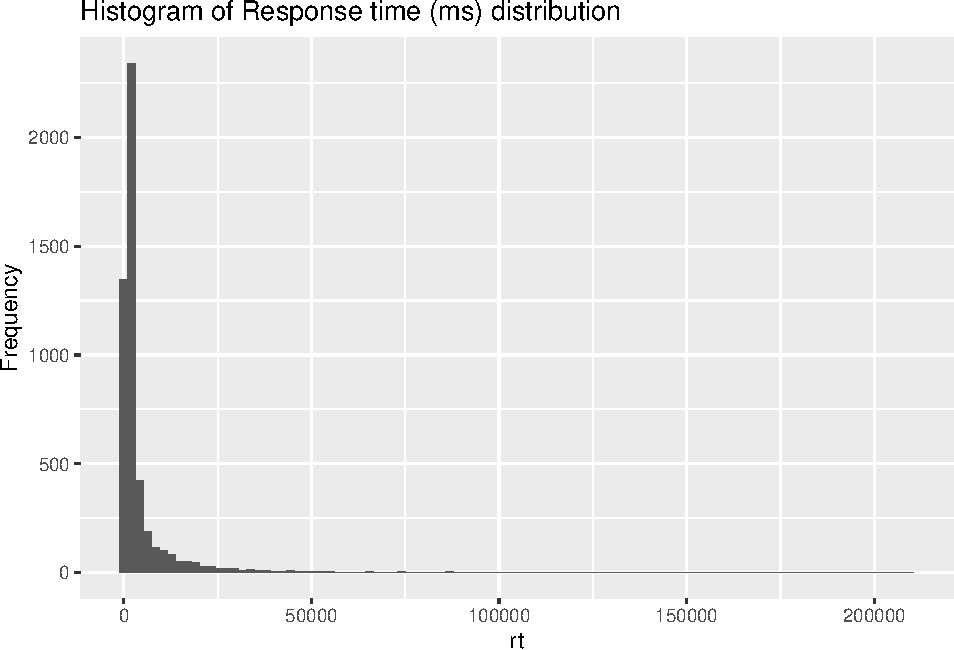
\includegraphics{L5_Checking_Assumptions_pdf_files/figure-latex/unnamed-chunk-13-1.pdf}

\hypertarget{cleaning}{%
\section{Cleaning}\label{cleaning}}

\begin{itemize}
\tightlist
\item
  Let's set the bounds that we had previously, between 500:5000 ms and
  take the log
\end{itemize}

\begin{Shaded}
\begin{Highlighting}[]
\NormalTok{df\_messy }\SpecialCharTok{|\textgreater{}}
  \FunctionTok{filter}\NormalTok{(rt }\SpecialCharTok{\%in\%} \FunctionTok{c}\NormalTok{(}\DecValTok{500}\SpecialCharTok{:}\DecValTok{5000}\NormalTok{)) }\SpecialCharTok{|\textgreater{}}
  \FunctionTok{ggplot}\NormalTok{(}\AttributeTok{mapping =} \FunctionTok{aes}\NormalTok{(}\FunctionTok{log}\NormalTok{(rt))) }\SpecialCharTok{+}
  \FunctionTok{geom\_histogram}\NormalTok{(}\AttributeTok{bins =} \DecValTok{100}\NormalTok{) }\SpecialCharTok{+} 
  \FunctionTok{labs}\NormalTok{(}\AttributeTok{y =} \StringTok{"Frequency"}\NormalTok{,}
       \AttributeTok{title =} \StringTok{"Histogram of log(rt) distribution"}\NormalTok{)}
\end{Highlighting}
\end{Shaded}

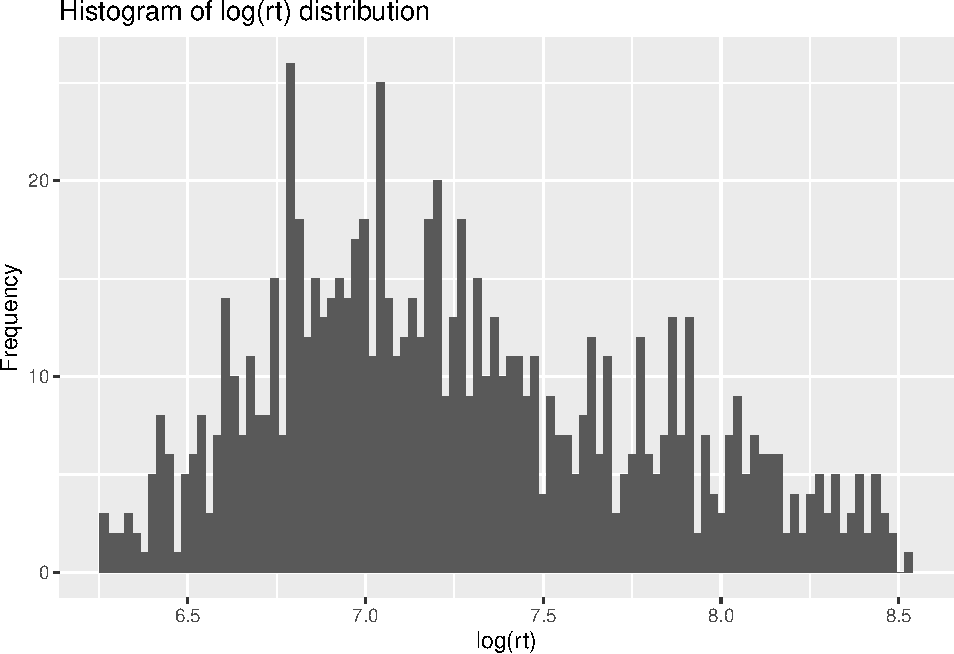
\includegraphics{L5_Checking_Assumptions_pdf_files/figure-latex/unnamed-chunk-14-1.pdf}

\hypertarget{calculate-the-mean-for-logrt}{%
\section{Calculate the mean for
log(rt)}\label{calculate-the-mean-for-logrt}}

\begin{Shaded}
\begin{Highlighting}[]
\NormalTok{df\_messy }\SpecialCharTok{|\textgreater{}}
  \FunctionTok{filter}\NormalTok{(rt }\SpecialCharTok{\%in\%} \FunctionTok{c}\NormalTok{(}\DecValTok{500}\SpecialCharTok{:}\DecValTok{5000}\NormalTok{)) }\SpecialCharTok{|\textgreater{}}
  \FunctionTok{summarise}\NormalTok{(}\AttributeTok{avg\_rt =} \FunctionTok{mean}\NormalTok{(rt))}
\end{Highlighting}
\end{Shaded}

\hypertarget{replace-missing-values-with-avg_rt}{%
\section{\texorpdfstring{Replace missing values with
\texttt{avg\_rt}}{Replace missing values with avg\_rt}}\label{replace-missing-values-with-avg_rt}}

\begin{Shaded}
\begin{Highlighting}[]
\CommentTok{\# Create mean variable}
\NormalTok{avg\_rt }\OtherTok{\textless{}{-}} \FloatTok{1646.523}

\CommentTok{\# create new object that replaces missing rt values with the mean}
\NormalTok{df\_messy1 }\OtherTok{\textless{}{-}}
\NormalTok{  df\_messy }\SpecialCharTok{|\textgreater{}}
  \FunctionTok{filter}\NormalTok{(rt }\SpecialCharTok{\%in\%} \FunctionTok{c}\NormalTok{(}\DecValTok{500}\SpecialCharTok{:}\DecValTok{5000}\NormalTok{)) }\SpecialCharTok{|\textgreater{}}              \CommentTok{\# remember to set the new bounds!}
  \FunctionTok{mutate}\NormalTok{(}\AttributeTok{rt =} \FunctionTok{if\_else}\NormalTok{(}\FunctionTok{is.na}\NormalTok{(rt), }
\NormalTok{                      avg\_rt, }\CommentTok{\# if the cell is empty, enter the mean of the vector}
\NormalTok{                      rt))                     }\CommentTok{\# otherwise, put what was there already }
\end{Highlighting}
\end{Shaded}

\hypertarget{examine-the-vector}{%
\section{Examine the vector}\label{examine-the-vector}}

\begin{Shaded}
\begin{Highlighting}[]
\CommentTok{\# Check for old}
\NormalTok{df\_messy }\SpecialCharTok{|\textgreater{}}
  \FunctionTok{summarise}\NormalTok{(}\AttributeTok{count\_nas =} \FunctionTok{is.na}\NormalTok{(rt) }\SpecialCharTok{|\textgreater{}}
              \FunctionTok{sum}\NormalTok{()) }\SpecialCharTok{|\textgreater{}}
  \FunctionTok{pluck}\NormalTok{(}\StringTok{"count\_nas"}\NormalTok{)}

\CommentTok{\# Check for new}
\NormalTok{df\_messy1 }\SpecialCharTok{|\textgreater{}}
  \FunctionTok{summarise}\NormalTok{(}\AttributeTok{count\_nas =} \FunctionTok{is.na}\NormalTok{(rt) }\SpecialCharTok{|\textgreater{}}
              \FunctionTok{sum}\NormalTok{()) }\SpecialCharTok{|\textgreater{}}
  \FunctionTok{pluck}\NormalTok{(}\StringTok{"count\_nas"}\NormalTok{)}
\end{Highlighting}
\end{Shaded}

\hypertarget{how-big-are-the-group-sizes-after-removing-missing-cases}{%
\section{How big are the group sizes after removing missing
cases?}\label{how-big-are-the-group-sizes-after-removing-missing-cases}}

\begin{Shaded}
\begin{Highlighting}[]
\CommentTok{\# What would I write here to check the group sizes?}
\end{Highlighting}
\end{Shaded}

\hypertarget{plot-the-data}{%
\section{Plot the data}\label{plot-the-data}}

\begin{Shaded}
\begin{Highlighting}[]
\NormalTok{df\_messy1 }\SpecialCharTok{|\textgreater{}}
  \FunctionTok{ggplot}\NormalTok{(}\AttributeTok{mapping =} \FunctionTok{aes}\NormalTok{(}\FunctionTok{log}\NormalTok{(rt))) }\SpecialCharTok{+}
  \FunctionTok{geom\_histogram}\NormalTok{(}\AttributeTok{bins =} \DecValTok{100}\NormalTok{) }\SpecialCharTok{+} 
  \FunctionTok{labs}\NormalTok{(}\AttributeTok{y =} \StringTok{"Frequency"}\NormalTok{,}
       \AttributeTok{title =} \StringTok{"Histogram of log(rt) distribution"}\NormalTok{)}
\end{Highlighting}
\end{Shaded}

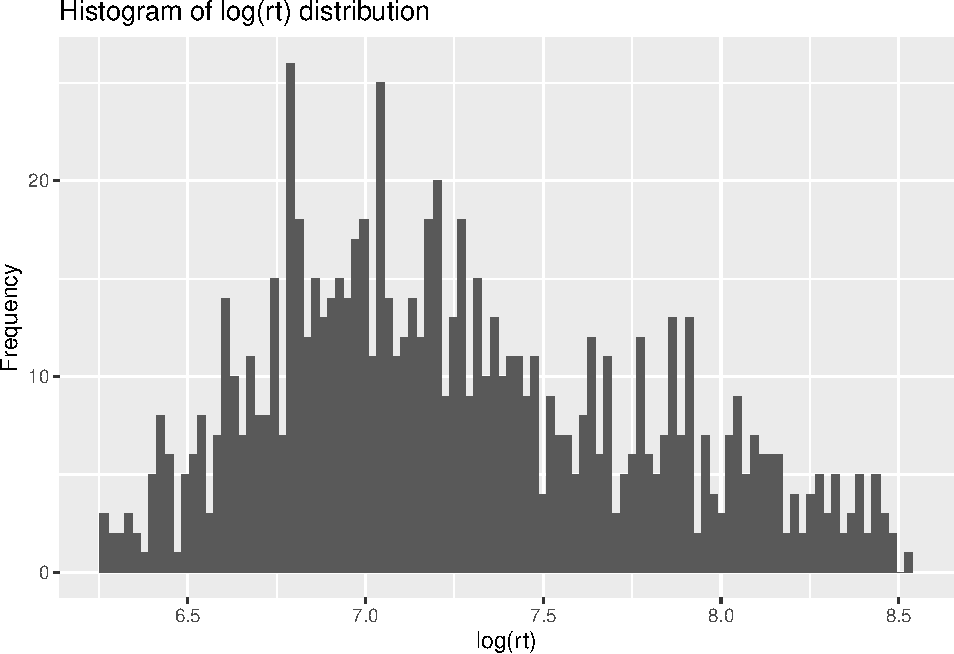
\includegraphics{L5_Checking_Assumptions_pdf_files/figure-latex/unnamed-chunk-19-1.pdf}

\hypertarget{tidyplots-equivalent}{%
\section{Tidyplots equivalent}\label{tidyplots-equivalent}}

\begin{Shaded}
\begin{Highlighting}[]
\CommentTok{\# using tidyplots}
\NormalTok{df\_messy1 }\OtherTok{\textless{}{-}}
\NormalTok{  df\_messy1 }\SpecialCharTok{|\textgreater{}}
  \FunctionTok{mutate}\NormalTok{(}\AttributeTok{log\_rt =} \FunctionTok{log}\NormalTok{(rt)) }\CommentTok{\# tidyplots needs to be passed existing vectors}

\NormalTok{df\_messy1 }\SpecialCharTok{|\textgreater{}}
  \FunctionTok{tidyplot}\NormalTok{(}\AttributeTok{x =}\NormalTok{ log\_rt, }\AttributeTok{color =}\NormalTok{ condition) }\SpecialCharTok{|\textgreater{}}
  \FunctionTok{add\_histogram}\NormalTok{(}\AttributeTok{bins =} \DecValTok{30}\NormalTok{) }\SpecialCharTok{|\textgreater{}} 
  \FunctionTok{add\_title}\NormalTok{(}\StringTok{"Histogram of log(rt) distribution per group"}\NormalTok{) }\SpecialCharTok{|\textgreater{}}
  \FunctionTok{adjust\_x\_axis\_title}\NormalTok{(}\StringTok{"log(rt)"}\NormalTok{) }\SpecialCharTok{|\textgreater{}}
  \FunctionTok{adjust\_y\_axis\_title}\NormalTok{(}\StringTok{"Frequency"}\NormalTok{)}
\end{Highlighting}
\end{Shaded}

\begin{center}\rule{0.5\linewidth}{0.5pt}\end{center}

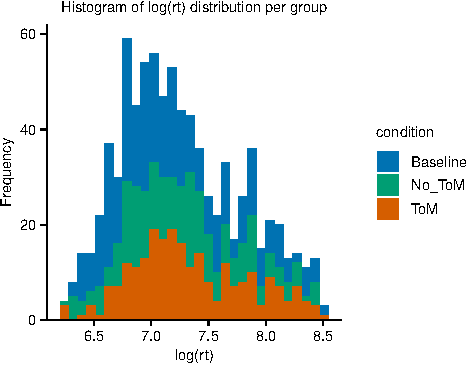
\includegraphics{L5_Checking_Assumptions_pdf_files/figure-latex/unnamed-chunk-21-1.pdf}

\hypertarget{checking-the-normality-of-the-data-using-psych}{%
\section{\texorpdfstring{Checking the normality of the data using
\texttt{psych}}{Checking the normality of the data using psych}}\label{checking-the-normality-of-the-data-using-psych}}

\begin{Shaded}
\begin{Highlighting}[]
\CommentTok{\# Overall}
\FunctionTok{describe}\NormalTok{(df\_messy1}\SpecialCharTok{$}\NormalTok{log\_rt) }\SpecialCharTok{|\textgreater{}}
  \FunctionTok{select}\NormalTok{(}\DecValTok{11}\NormalTok{,}\DecValTok{12}\NormalTok{)}

\CommentTok{\# By group}
\FunctionTok{describeBy}\NormalTok{(log\_rt }\SpecialCharTok{\textasciitilde{}}\NormalTok{ condition,}
           \AttributeTok{mat =} \ConstantTok{TRUE}\NormalTok{,}
           \AttributeTok{data =}\NormalTok{ df\_messy1) }\SpecialCharTok{|\textgreater{}}
  \FunctionTok{select}\NormalTok{(}\DecValTok{2}\NormalTok{, }\DecValTok{13}\SpecialCharTok{:}\DecValTok{14}\NormalTok{)}
\end{Highlighting}
\end{Shaded}

\begin{itemize}
\tightlist
\item
  What is \texttt{select} doing here?
\item
  What are the rules for violations to Skew and Kurtosis?
\end{itemize}

\hypertarget{boxplot-with-comparison-analysis-from-tidyplots}{%
\section{\texorpdfstring{Boxplot with comparison analysis from
\texttt{tidyplots}}{Boxplot with comparison analysis from tidyplots}}\label{boxplot-with-comparison-analysis-from-tidyplots}}

\begin{Shaded}
\begin{Highlighting}[]
\NormalTok{df\_messy1 }\SpecialCharTok{|\textgreater{}} 
  \FunctionTok{tidyplot}\NormalTok{(}\AttributeTok{x =}\NormalTok{ condition, }
           \AttributeTok{y =}\NormalTok{ log\_rt, }
           \AttributeTok{color =}\NormalTok{ condition) }\SpecialCharTok{|\textgreater{}} 
  \FunctionTok{add\_boxplot}\NormalTok{() }\SpecialCharTok{|\textgreater{}} 
  \FunctionTok{add\_test\_pvalue}\NormalTok{(}\AttributeTok{ref.group =} \DecValTok{1}\NormalTok{) }\SpecialCharTok{|\textgreater{}}
  \FunctionTok{add\_title}\NormalTok{(}\StringTok{"Comparing log(rt) against the baseline"}\NormalTok{) }\SpecialCharTok{|\textgreater{}}
  \FunctionTok{adjust\_x\_axis\_title}\NormalTok{(}\StringTok{"Experimental group"}\NormalTok{) }\SpecialCharTok{|\textgreater{}}
  \FunctionTok{adjust\_y\_axis\_title}\NormalTok{(}\StringTok{"log(rt)"}\NormalTok{) }\SpecialCharTok{|\textgreater{}}
  \FunctionTok{adjust\_legend\_title}\NormalTok{(}\StringTok{"Experimental group"}\NormalTok{)}
\end{Highlighting}
\end{Shaded}

\begin{center}\rule{0.5\linewidth}{0.5pt}\end{center}

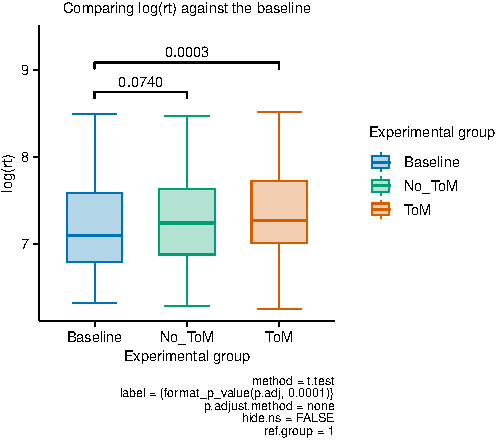
\includegraphics{L5_Checking_Assumptions_pdf_files/figure-latex/unnamed-chunk-24-1.pdf}

\hypertarget{roundup}{%
\section{Roundup}\label{roundup}}

\begin{itemize}
\tightlist
\item
  I showed you how to deliberately untidy data using the
  \textbf{\texttt{messy}} package
\item
  We did some label tidying
\item
  We examined the case of listwise deletion, with your reading covering
  other approaches to missing data
\item
  We examined test statistics for distribution normality
\item
  Gave you a fist look at \textbf{\texttt{tidyplots}} as an alternative
  to \textbf{\texttt{ggplot2}}
\end{itemize}

\hypertarget{cleanup}{%
\section{Cleanup}\label{cleanup}}

\begin{Shaded}
\begin{Highlighting}[]
\CommentTok{\# Clear data}
\FunctionTok{rm}\NormalTok{(}\AttributeTok{list =} \FunctionTok{ls}\NormalTok{())  }\CommentTok{\# Removes all objects from environment}

\CommentTok{\# Clear packages}
\FunctionTok{p\_unload}\NormalTok{(all)  }\CommentTok{\# Remove all contributed packages}

\CommentTok{\# Clear plots}
\FunctionTok{graphics.off}\NormalTok{()  }\CommentTok{\# Clears plots, closes all graphics devices}

\CommentTok{\# Clear console}
\FunctionTok{cat}\NormalTok{(}\StringTok{"}\SpecialCharTok{\textbackslash{}014}\StringTok{"}\NormalTok{)  }\CommentTok{\# Mimics ctrl+L}
\end{Highlighting}
\end{Shaded}

\hypertarget{references}{%
\section{References}\label{references}}

\end{document}
